\documentclass[a4paper,11pt]{article}

%%%%%%%%%%%%%%%%%%%%%%%%%%%%%%%%%%%%%%%%%%%%%%%%%%%%%%%%%%%%%%%%%%%%%%%%
% Paquetes utilizados
%%%%%%%%%%%%%%%%%%%%%%%%%%%%%%%%%%%%%%%%%%%%%%%%%%%%%%%%%%%%%%%%%%%%%%%%

% Graficos complejos
\usepackage{graphicx}
\usepackage{caption}
\usepackage{subcaption}
\usepackage{placeins}

% Soporte para el lenguaje español
\usepackage{textcomp}
\usepackage[utf8]{inputenc}
\usepackage[T1]{fontenc}
\DeclareUnicodeCharacter{B0}{\textdegree}
\usepackage[spanish]{babel}

% Codigo fuente embebido
\usepackage{listings}

% PDFs embebidos para el apendice
\usepackage{pdfpages}

% Matematicos
\usepackage{amssymb,amsmath}

% Tablas complejas
\usepackage{multirow}

% Fromato MIPS para los archivos incluidos
\usepackage{docs/mips}

% Formato de parrafo
\setlength{\parskip}{1ex plus 0.5ex minus 0.2ex}

%%%%%%%%%%%%%%%%%%%%%%%%%%%%%%%%%%%%%%%%%%%%%%%%%%%%%%%%%%%%%%%%%%%%%%%%
% Titulo
%%%%%%%%%%%%%%%%%%%%%%%%%%%%%%%%%%%%%%%%%%%%%%%%%%%%%%%%%%%%%%%%%%%%%%%%

% Titulo principal del documento.
\title{\textbf{Trabajo Practico 1: Conjunto de Instrucciones MIPS}}

% Informacion sobre los autores.
\author{\\
  Guido Laghi, \textit{P. 82.449}                                  \\
  \texttt{guido321@gmail.com}                                      \\ [2.5ex]
  Sebastian L. Perez, \textit{P. 84.379}                           \\
  \texttt{sebastian.leo.perez@gmail.com}                           \\ [2.5ex]
  Sergio Matias Piano, \textit{P. 85.191}                          \\
  \texttt{smpiano@gmail.com}                                       \\ [2.5ex]
                                                                   \\
  \normalsize{1er. Cuatrimestre de 2013}                           \\
  \normalsize{66.20 Organizacion de Computadoras}                  \\
  \normalsize{Facultad de Ingenieria, Universidad de Buenos Aires} \\
}
\date{}

%%%%%%%%%%%%%%%%%%%%%%%%%%%%%%%%%%%%%%%%%%%%%%%%%%%%%%%%%%%%%%%%%%%%%%%%
% Documento
%%%%%%%%%%%%%%%%%%%%%%%%%%%%%%%%%%%%%%%%%%%%%%%%%%%%%%%%%%%%%%%%%%%%%%%%

\begin{document}

% ----------------------------------------------------------------------
% Top matter
% ----------------------------------------------------------------------
\thispagestyle{empty}
\maketitle

\begin{abstract}

  Este informe sumariza el desarrollo del trabajo practico 1 de la materia
  Organizacion de Computadoras (66.20) dictada en el primer cuatrimestre de
  2013 en la Facultad de Ingenieria de la Universidad de Buenos Aires. El mismo
  consiste en la construccion de un sistema minimalista de ordenamiento de
  archivos y el analisis de performance y perfilado del mismo.

\end{abstract}

\clearpage

% ----------------------------------------------------------------------
% Tabla de contenidos
% ----------------------------------------------------------------------
\tableofcontents
\clearpage


% ----------------------------------------------------------------------
% Desarrollo
% ----------------------------------------------------------------------
\part{Desarrollo}

\section{Introduccion}

  El objetivo de este trabajo es comparar el rendimiento que tienen dos
  algoritmos de ordenamiento escritos en C. Sabemos por experiencia que
  un ordenamiento (Shell) es mejor que el otro (Bubble). Luego el objetivo
  es evaluar cómo cambia el rendimiento cuando el código está escrito
  directamente en codigo assembly de MIPS.

  Esta alternativa tiene una caracteristica fundamental: al tener
  acceso al conjunto de instrucciones que ejecuta la arquitectura potencialmente
  se puede desarrollar una solucion optima, minimizando el acceso a memoria, la
  cantidad de instrucciones a ejecutar, etc.

  Por otro lado, la implementacion en assembly de un sistema no trivial es una
  tarea complicada. La dificultad principal radica en que es tarea del
  programador implementar y controlar muchos de los mecanismos de bajo nivel que
  constituyen el \textit{como} de la solucion, en vez de concentrarse en el
  \textit{que}. Algunos ejemplos son el manejo del stack, la implementacion de
  convenciones de llamadas de subrutinas, el uso de registros compartidos, entre
  otros.

\section{Implementacion}

  El sistema que resuelve el problema planteado en el enunciado (disponible en el
  anexo~\ref{sec:enunciado}) fue implementado mayoritariamente en C, y parte en
  lenguaje MIPS como lo indicaba el enunciado. La diferencia fundamental radica 
  en la implementacion de las rutinas de ordenamiento a traves del algoritmo
  \textit{shellsort} directamente en assembly. El codigo fuente de
  la solucion esta disponible en el anexo~\ref{sec:source}; que a continuación
  se incluyen los archivos fuentes relacionados con la implementación en
  lenguaje assembly de la solucion desarrollada.

  Cabe destacar que la solucion en assembly definitivamente no es la solucion
  optima. Hemos realizado algunas mejoras respecto de la version inicial como
  quitar el \textit{Área Desconocida} de la memoria (ya que por error nuestro la 
  incluimos en la primer entrega), y la implementacion de los metodos de swap 
  y comparación sin tener en cuenta el case de la palabra en codigo MIPS 
  (antes usabamos desde MIPS las escritas en leguaje C o bien llamadas a librerías).
  A continuacion enumeraremos algunas consideraciones de diseño tomadas al
  implementar cada una de las funciones involucradas en el algoritmo de
  ordenamiento.

\subsection{shell\_sort\_S}

  Esta funcion implementa el ordenamiento de una tabla de strings (de palabras)
  a traves del algoritmo de ordenamiento \textit{shellsort}. El metodo de 
  ordenamiento fue implementado en su forma mas sencilla a traves de un 
  algoritmo iterativo. El stack frame utilizado para la función se describe 
  en la figura~\ref{fig:stack_shell_sort}.

\begin{figure}[h!]
  \centering
  \includegraphics[scale=0.75]{docs/stack_shell.png}
  \caption{Stack de shell sort implementado por nosotros en MIPS}
  \label{fig:stack_shell_sort}
\end{figure}

\begin{figure}[h!]
  \centering
  \includegraphics{docs/stack_compare_s.png}
  \caption{Stack de la función compare sin case}
\end{figure}

\begin{figure}[h!]
  \centering
  \includegraphics{docs/stack_swap_s.png}
  \caption{Stack de la función swap}
\end{figure}

\FloatBarrier

  Se reservan 32 bytes para el area de SRA: 4 bytes para salvar el registro \textit{ra}
  en llamadas a otras funciones (ya que no es leaf), 4 bytes para salvar el
  registro þ\textit{gp}, 4 bytes para preservar el registro fp y finalmente 20
  bytes para el uso interno de los registros S0, S1, S2, S3, S4 que se utilizan
  para calculos de la funcion.

  Por otro lado, dado que las funciones invocadas desde esta no poseen nunca mas
  de dos argumentos, se reservan \(4 x 4\) bytes en concepto de ABA (respetando
  la ABI) para ser utilizados por las funciones llamadas.

\FloatBarrier

\section{Compilacion}

  Se instrumento un \textit{makefile} para ejecutar las instrucciones adecuadas
  de compilacion para los distintos escenarios requeridos. La
  tarea \textit{make} compila individualmente cada uno de los archivos fuente de
  extension \textit{c} y \textit{S} a traves del ejecutable \textit{gcc}.
  Los comandos utilizados para compilar cada uno de estos archivos fuente son los
  siguientes:

\begin{lstlisting}
  gcc -c -o build/obj/buffer.o source/buffer.c 
                  -I./source -Wall
  gcc -c -o build/obj/data.o source/data.c 
                  -I./source -Wall
  gcc -c -o build/obj/clargs.o source/clargs.c 
                  -I./source -Wall
  gcc -c -o build/obj/cltext.o source/cltext.c 
                  -I./source -Wall
  gcc -c -o build/obj/tp1.o source/tp1.c -I./source 
                  -Wall
  gcc -c -o build/obj/bubblesort.o source/bubblesort.c 
                  -I./source -Wall
  gcc -c -o build/obj/shellsort.o source/shellsort.c 
                  -I./source -Wall
\end{lstlisting}

  De este listado, cada una de las invocaciones obedece a la siguiente estructura
  de argumentos:

\begin{description}

  \item[-c] Compila o ensambla el codigo fuente pero no corre el linker.  Por
    lo tanto la salida corresponde a un archivo objeto por cada archivo fuente.

  \item[-o] Especifica cual sera el archivo de salida sea este un archivo
    objeto, ejecutable, ensamblado o codigo preprocesado de C.

  \item[-Wall] Activa todos los mensajes de warning.

  \item[-I] Agrega el directorio especificado a la lista de directorios
    buscados para los archivos header

\end{description}

  El resultado de la ejecucion de estos comandos es que se generan archivos
  objeto para cada fuente, listos para ser linkeados, en el directorio
  \textit{build/obj}. Para realizar este ultimo paso, se invoca nuevamente a
  \textit{gcc} con un ultimo comando:

\begin{lstlisting}
  gcc -o build/tp1 build/obj/buffer.o 
  build/obj/data.o 
  build/obj/clargs.o 
  build/obj/cltext.o 
  build/obj/tp1.o 
  build/obj/bubblesort.o 
  build/obj/shellsort.o 
    -I./source -Wall 
\end{lstlisting}

  El comando linkea todos los archivos objeto en un ejecutable final,
  \textit{build/tp1}.

\section{Analisis de tiempos de ejecucion}

  En las siguientes secciones detallaremos el proceso de analisis de tiempo de
  ejecucion realizado para los diferentes casos contemplados.

\subsection{Analisis previo}\label{sec:tiempos}

  El analisis de tiempos de ejecucion se focalizara en comparar la performance de
  la implementacion en assembly descripta anteriormente contra diferentes
  versiones de esencialmente el mismo sistema.

  Primero se comparara el desempeño de los algoritmos escritos en C. utilizando
  todas las optimizaciones disponibles por el compilador. Se espera nuevamente
  encontrar algunas mejoras, aunque pequeñas, con respecto a lo que puede
  entregar el compilador.

  Luego se comparara el algoritmo escrito en C contra el mismo en lenguaje ensabmblador.
  Por un lado, al compilar esta solucion sin ninguna optimizacion del compilador
  se espera obtener ganancias de performance apreciables, debidas mayormente al
  mejor manejo de los accesos a memoria logrados por el ejecutable desarrollado
  en assembly.

\subsection{Experimentos}

  Se realizaron pruebas utilizando los archivos provistos por la catedra sobre un
  entorno de ubuntu actual y sobre el emulador GXemul.
  Obtuvimos los siguientes resultados (tiempo usr + real)

\FloatBarrier

\begin{table}[h!t]
\centering
\begin{tabular}{| l | r |}
  \hline
  Archivo           & Tiempo de ejecucion \\ \hline
  Alice             & \(3.028s\) \\
  Beowulf           & \(3.914s\) \\
  Cyclopedia        & \(13.352s\) \\
  EL Quijote        & \(57.008s\) \\
  \hline
\end{tabular}

\caption{Tiempos para ShellSort}
\label{tab:resultados}
\end{table}

\FloatBarrier

\begin{table}[h!t]
\centering
\begin{tabular}{| l | r |}
  \hline
  Archivo           & Tiempo de ejecucion \\ \hline
  Alice             & \(10m18.336s\) \\
  Beowulf           & \(16m59.469s\) \\
  Cyclopedia        & \(133m52.200s\) \\
  EL Quijote        & \textit{mas de 1 dia} \\
  \hline
\end{tabular}
\caption{Tiempos para BubbleSort}
\label{tab:resultados}
\end{table}

\FloatBarrier

  Como se esperaba, el codigo de shellsort anduvo muchisimo mejor que el bubble,
  tardando incluso menos de 1 minuto en ordenar. En cambio el bubblesort tardo
  excesivo tiempo en completarse, al punto que el archivo "Quijote" excedio
  nuestro tiempo de medicion maximo establecido (1 dia).

\section{Conclusiones}

  La implementacion en assembly del trabajo practico, a pesar de que los
  algoritmos son relativamente simples y sencillos de desarrollar, fue
  mucho mas complicado y tedioso.
  Analizando el resto de los resultados concluimos que la version implementada en
  C con \textit{shellsort}, incluso cuando no se aplicaron optimizaciones de
  compilador, era un orden de magnitud mas eficiente que la version implementada
  en assembly.

  Como conclusion final podemos decir que si bien la implementacion de MIPS nos
  ofrece un mejor rendimiento de los algoritmos desarrollados, su dificil
  implementacion hace que debamos evaluar si deseamos priorizar el rendimiento
  a costo de tiempo de desarrollo. En caso de necesitar una mejora crucial de
  rendimiento la mejor solucion es la arquitectura MIPS, mientras que si deseamos
  un desarrollo mas sencillo (y por lo tanto mas breve) la mejor opcion es
  lenguaje en C.

  Respecto a los tiempos de medicion, podemos concluir que sin ningun lugar a
  dudas usariamos el shellsort para ordenar, ya que gana muchisimo en rendmiento
  respecto del bubblesort. El bubblesort aumenta muchisimo el tiempo de ejecucion
  cuando aumenta el tamaño del archivo a medir, y no pasa tanto asi con el otro
  algoritmo. Desde ya que no podemos esperar un dia entero a que ordene un archivo,
  por mas simple que sea la implementacion del mismo.

\clearpage

\part{Apendice}
\appendix

\section{Enunciado original}\label{sec:enunciado}
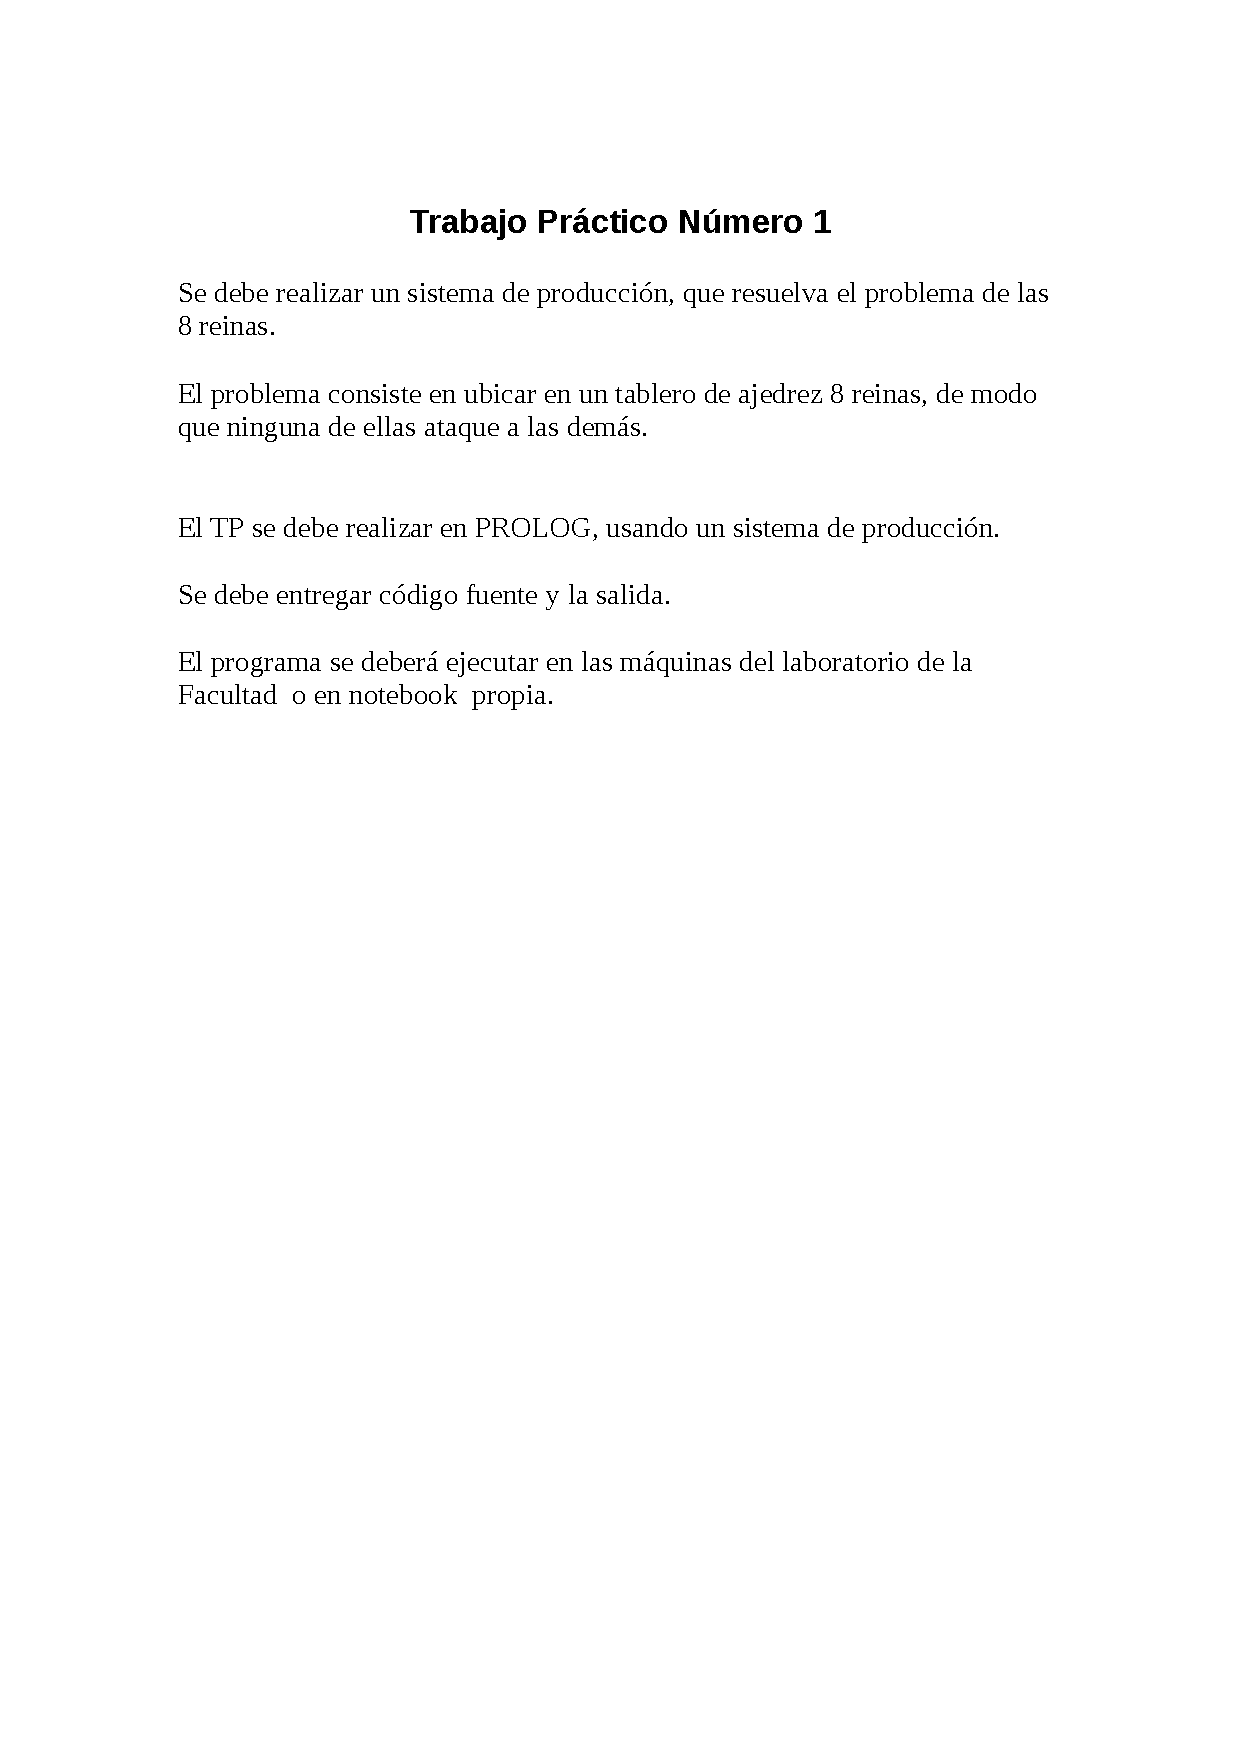
\includepdf[pages={-}]{docs/enunciado.pdf}

\clearpage
\section{Codigo fuente}\label{sec:source}
\clearpage
\definecolor{gray}{rgb}{0.5,0.5,0.5}
\lstset{%
  title=\lstname,
  language=C,
  basicstyle=\footnotesize,
  showspaces=false,
  showstringspaces=false,
  breaklines=true,
  commentstyle=\color{gray},
  numbers=left,
  numberstyle=\tiny\color{gray},
  numbersep=5pt,
  frame=single
}

\lstinputlisting{source/bubblesort.c}
\lstinputlisting{source/bubblesort.h}
\lstinputlisting{source/buffer.c}
\lstinputlisting{source/buffer.h}
\lstinputlisting{source/clargs.c}
\lstinputlisting{source/clargs.h}
\lstinputlisting{source/cltext.c}
\lstinputlisting{source/cltext.h}
\lstinputlisting{source/config.h}
\lstinputlisting{source/data.c}
\lstinputlisting{source/data.h}
\lstinputlisting{source/shellsort.c}
\lstinputlisting{source/shellsort.h}
\lstinputlisting{source/tp1.c}
\lstset{%
  language=[mips]Assembler,       % the language of the code
  basicstyle=\footnotesize,       % the size of the fonts that are used for the code
  numbers=left,                   % where to put the line-numbers
  numberstyle=\tiny\color{gray},  % the style that is used for the line-numbers
  stepnumber=1,                   % the step between two line-numbers. If it's 1, each line 
                                  % will be numbered
  numbersep=5pt,                  % how far the line-numbers are from the code
  backgroundcolor=\color{white},  % choose the background color. You must add \usepackage{color}
  showspaces=false,               % show spaces adding particular underscores
  showstringspaces=false,         % underline spaces within strings
  showtabs=false,                 % show tabs within strings adding particular underscores
  frame=single,                   % adds a frame around the code
  rulecolor=\color{black},        % if not set, the frame-color may be changed on line-breaks within not-black text (e.g. commens (green here))
  tabsize=4,                      % sets default tabsize to 2 spaces
  captionpos=b,                   % sets the caption-position to bottom
  breaklines=true,                % sets automatic line breaking
  breakatwhitespace=false,        % sets if automatic breaks should only happen at whitespace
  title=\lstname,                 % show the filename of files included with \lstinputlisting;
                                  % also try caption instead of title
  keywordstyle=\color{blue},      % keyword style
  commentstyle=\color{green},     % comment style
  stringstyle=\color{red},      % string literal style
  escapeinside={\%*}{*)},         % if you want to add a comment within your code
  morekeywords={*}                % if you want to add more keywords to the set
}
\lstinputlisting{source/shellsort.S}

\clearpage
\section{Toma de tiempos en bruto}\label{sec:enunciado}
\lstinputlisting{docs/tiempos.txt}

\end{document}
